\begin{equation}
    \begin{gathered}
        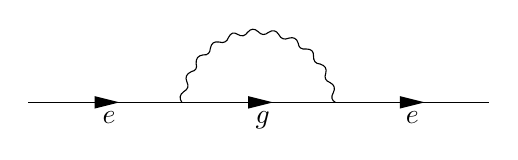
\begin{tikzpicture}[x=0.75pt,y=0.75pt,yscale=-1,xscale=1]
            %uncomment if require: \path (0,300); %set diagram left start at 0, and has height of 300
            
            %Straight Lines [id:da01124014261520312] 
            \draw    (79,179) -- (153,179) ;
            %Straight Lines [id:da5714521171594549] 
            \draw    (118,179) -- (121,179) ;
            \draw [shift={(123,179)}, rotate = 180] [fill={rgb, 255:red, 0; green, 0; blue, 0 }  ][line width=0.08]  [draw opacity=0] (12,-3) -- (0,0) -- (12,3) -- cycle    ;
            %Straight Lines [id:da7252034130949252] 
            \draw    (153,179) -- (227,179) ;
            %Straight Lines [id:da483809936593951] 
            \draw    (192,179) -- (195,179) ;
            \draw [shift={(197,179)}, rotate = 180] [fill={rgb, 255:red, 0; green, 0; blue, 0 }  ][line width=0.08]  [draw opacity=0] (12,-3) -- (0,0) -- (12,3) -- cycle    ;
            %Curve Lines [id:da12282081273981671] 
            \draw    (153,179) .. controls (151.65,176.93) and (151.97,175.2) .. (153.97,173.82) .. controls (156.01,172.68) and (156.49,171.09) .. (155.42,169.06) .. controls (154.49,166.91) and (155.2,165.3) .. (157.57,164.21) .. controls (159.74,163.75) and (160.52,162.46) .. (159.9,160.35) .. controls (159.69,157.84) and (160.83,156.44) .. (163.3,156.13) .. controls (165.45,156.34) and (166.6,155.26) .. (166.77,152.9) .. controls (167.19,150.49) and (168.6,149.51) .. (170.99,149.95) .. controls (173.22,150.62) and (174.74,149.87) .. (175.53,147.68) .. controls (176.58,145.51) and (178.01,145.02) .. (179.82,146.21) .. controls (181.78,147.46) and (183.42,147.13) .. (184.74,145.22) .. controls (186.31,143.39) and (187.98,143.29) .. (189.75,144.91) .. controls (191.3,146.64) and (192.98,146.76) .. (194.77,145.28) .. controls (196.78,143.95) and (198.42,144.3) .. (199.71,146.33) .. controls (200.76,148.42) and (202.35,149.01) .. (204.5,148.08) .. controls (206.83,147.36) and (208.35,148.17) .. (209.07,150.51) .. controls (209.26,152.64) and (210.54,153.57) .. (212.91,153.29) .. controls (215.4,153.28) and (216.57,154.39) .. (216.44,156.63) .. controls (216.34,159.07) and (217.39,160.37) .. (219.6,160.53) .. controls (222.08,161.28) and (222.99,162.77) .. (222.34,165) .. controls (221.53,167.14) and (222.21,168.62) .. (224.37,169.45) .. controls (226.52,170.52) and (227.06,172.16) .. (225.97,174.35) .. controls (224.76,176.44) and (225.11,177.99) .. (227,179) -- (227,179) ;
            %Straight Lines [id:da2752757330155595] 
            \draw    (227,179) -- (301,179) ;
            %Straight Lines [id:da34684664641318586] 
            \draw    (265,179) -- (268,179) ;
            \draw [shift={(270,179)}, rotate = 180] [fill={rgb, 255:red, 0; green, 0; blue, 0 }  ][line width=0.08]  [draw opacity=0] (12,-3) -- (0,0) -- (12,3) -- cycle    ;
            
            % Text Node
            \draw (118,182.4) node [anchor=north] [inner sep=0.75pt]    {$e$};
            % Text Node
            \draw (192,182.4) node [anchor=north] [inner sep=0.75pt]    {$g$};
            % Text Node
            \draw (264,182.4) node [anchor=north] [inner sep=0.75pt]    {$e$};
            \end{tikzpicture}
    \end{gathered},
    \label{eq:one-loop}
\end{equation}